\documentclass{article}

\usepackage{lmodern}
\usepackage[T1]{fontenc}
\usepackage[spanish,activeacute]{babel}
\usepackage{mathtools}
\usepackage[utf8]{inputenc}
\usepackage{enumerate}
\usepackage[a4paper, total={7in, 11in}]{geometry}
\usepackage{graphicx}
\usepackage{charter}

\begin{document}
\begin{center}
\large \textbf{Práctica 6}: Lenguajes formales y gramáticas
\end{center}
\graphicspath{ {./img/} }
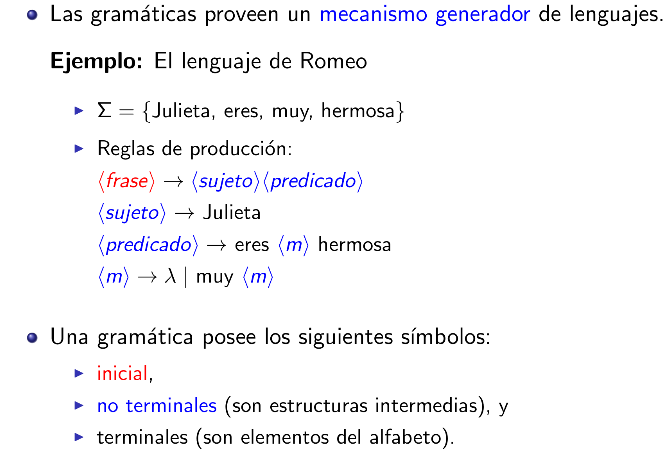
\includegraphics[scale=0.4]{1.png} \\ \\
\textbf{Definición: Gramática} es una tupla: $(N,T,P,\sigma)$ donde: \\
\begin{itemize}
  \item
    N es un conjunto finito de símbolos llamados \textbf{no terminantes}.
  \item
    T es un conjunto finito de símbolos, llamados \textbf{terminantes} o \textbf{alfabeto},
    tal que $N \cap T = \emptyset$
  \item
    P es un conjunto finito de \textbf{reglas de producción}, donde
    \[ P \subseteq ((N \cup T)^{*} - T^{*}) \times (N \cup T)^{*}\]
    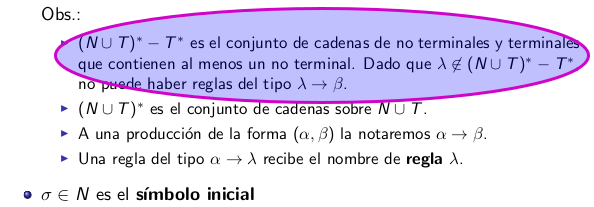
\includegraphics[scale=0.5]{4.png} \\
    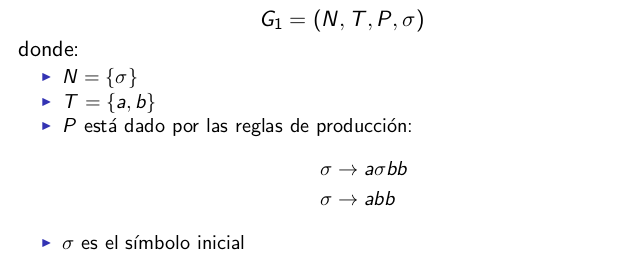
\includegraphics[scale=0.5]{5.png}
\end{itemize}
\textbf{Definición 1.} Una gramática se dice:
\begin{enumerate}[(a)]
\item
    \textit{regular} si cada producción es de la forma:
    $A \rightarrow a$ o $A \rightarrow aB$ o $A \rightarrow \lambda \quad$ 
    donde $A, B \in N$ y $a \in T$, \\ \\ \\
    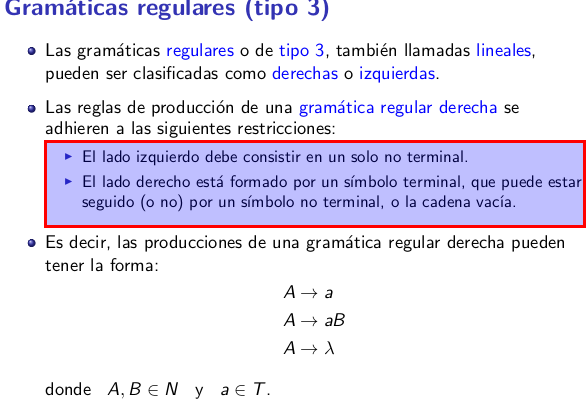
\includegraphics[scale=0.4]{3.png}
    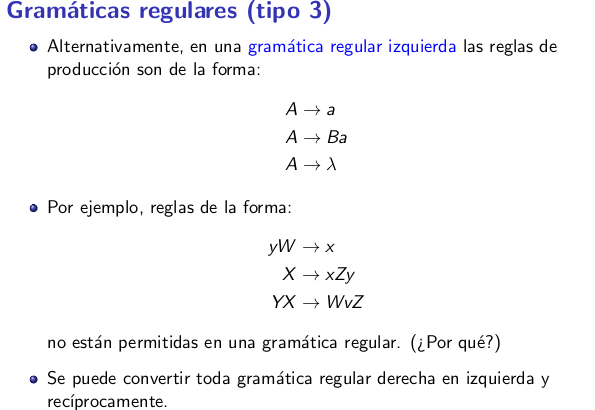
\includegraphics[scale=0.4]{2.png} \\ \\ \\ \\ \\ \\
\item
    \textit{libre} (o independiente) de contexto si cada producción es de la forma 
    $A \rightarrow \delta$ donde $A \in N$ y $\delta \in (N \cup T)^*$ o 
    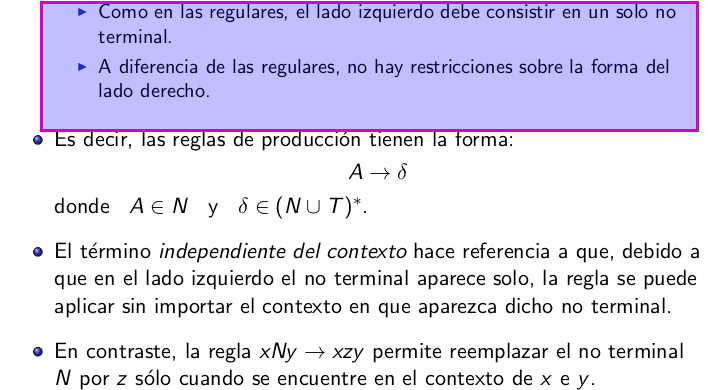
\includegraphics[scale=0.5]{6.png}
\item
  \textit{sensible al contexto} si cada producción es de la forma
    $aA\beta \rightarrow \alpha\delta\beta$ donde $A \in N, \alpha,\beta \in (N \cup T)^*$ y $\delta \in (N \cup T)^+$,
\item
    \textit{estructurada} por frases o irrestricta si no tiene restricciones sobre la forma de sus producciones, es decir
   si son de la forma
    \[ \alpha \rightarrow \delta \text{\quad donde \quad} \alpha \in (N \cup T)^* - T^* \quad y \quad \delta \in (N \cup T)^* \]
\end{enumerate}

\begin{enumerate}[1.]
\item
Clasifique cada una de las siguientes gramáticas (dando su tipo más restrictivo):
  \begin{enumerate}[a)]
    \item
      $T = \{ a,b\}, N = \{ \sigma, A\}$, símbolo inicial $\sigma$, y producciones
      \[ \sigma \rightarrow b\sigma, \sigma \rightarrow aA, A \rightarrow a\sigma,\]
      \[ A \rightarrow bA, A \rightarrow a, \sigma \rightarrow b\]
      Regular.
    \item 
      $T = \{ a,b,c \}, N = \{ \alpha,A,B\}$, símbolo inicial $\sigma$, y producciones
      \[ \sigma \rightarrow AB, AB \rightarrow BA, A \rightarrow aA,\]
      \[ B \rightarrow Bb, A \rightarrow a, B \rightarrow b\] \\
       Sensible al contexto.
    \item
      $T = \{ a,b\}, N = \{ \sigma, A,B\}$, śimbolo inicial $\sigma$ y producciones:
      \[ \sigma \rightarrow A, \quad \sigma \rightarrow AAB,\quad Aa \rightarrow ABa, \quad A \rightarrow aa,\]
      \[ Bb \rightarrow ABb, \quad AB \rightarrow ABB, \quad B \rightarrow b.\]
      Sensible al contexto.
    \item
      $T = \{ a,b,c \}, N = \{\sigma,A,B \},$ símbolo inicial $\sigma$, y producciones:
      \[ \sigma \rightarrow BAB, \quad \sigma \rightarrow ABA, \quad A \rightarrow AB, \quad B \rightarrow BA,\]
      \[A \rightarrow aA, \quad A ab, \quad B \rightarrow b.\]
      Independiente de contexto.
  \end{enumerate}
\end{enumerate}
\end{document}
